\iffalse
\documentclass{article}
\usepackage{amsmath}
\usepackage{xcolor}
\usepackage{gensymb}
\usepackage{ragged2e}
\usepackage{graphicx}
\usepackage{gensymb}
\usepackage{mathtools}
\newcommand{\mydet}[1]{\ensuremath{\begin{vmatrix}#1\end{vmatrix}}}
\providecommand{\brak}[1]{\ensuremath{\left(#1\right)}}
\providecommand{\norm}[1]{\left\lVert#1\right\rVert}
\newcommand{\solution}{\noindent \textbf{Solution: }}
\newcommand{\myvec}[1]{\ensuremath{\begin{pmatrix}#1\end{pmatrix}}}
\let\vec\mathbf
\begin{document}
\begin{center}
        \textbf\large{CHAPTER-7 \\ TRIANGLES}
\end{center}
\section{Exercise 7.1}
Q1. \textbf{Construction}\\
\fi
See 
	  \tabref{tab:9/7/1/1/Table1}.
\begin{figure}[H]
	\begin{center}
		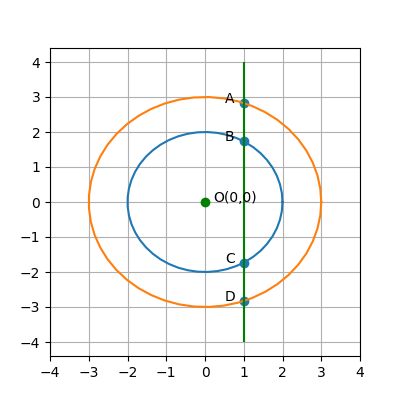
\includegraphics[width=0.75\columnwidth]{chapters/9/7/1/1/figs/fig.png}
	\end{center}
	\caption{Quadrilateral CBAD}
	\label{fig:chapters/9/7/1/1/Fig1}
\end{figure}
\begin{table}[H]
	  \centering
	  \begin{tabular}{|p{3cm}|p{3cm}|p{3cm}|}
\hline                                        
\textbf{Symbol} & \textbf{Values} & \textbf{Description}\\                                          
\hline                                 
$\theta$ & 30$\degree{}$   & $\angle{BAD} = \angle{BAC}$ \\           
\hline                                    
a &  9 & $AB$ \\     
\hline                      
c & 5 & $AC$ \\
\hline                                     
		$\vec{e}_1$ & $\myvec{
			1\\
			0\\
			}$ & basis vector\\ 
\hline
\end{tabular}

	  \caption{Parameters}
	  \label{tab:9/7/1/1/Table1}
\end{table}
The vertices of the quadrilateral can be expressed as
\begin{align}
	\vec{A} = \myvec{0\\0},\vec{B} = a\vec{e_1},\vec{C} = \myvec{c\cos\theta\\c\sin\theta},\vec{D} = \myvec{c\cos\theta\\-c\sin\theta}
\end{align}
where
\begin{align}
	\vec{C}-\vec{A} &= \vec{A}-\vec{D}\\
	\angle{CAB} &= \angle{DAB}
\end{align}
\begin{align}
	AB:	\vec{n}^{\top}\vec{x} = 0,
\end{align}
where
\begin{align}
\vec{n} = \myvec{0\\1}
\end{align}
Letting
		\begin{align}
\theta_1=&\angle CBA 
		\end{align}
		and substituting numerical values,
		\begin{align}
\vec{m_1}=&\vec{B}-\vec{C}=\myvec{4.7\\-2.5}, \vec{m_2}=\vec{B}-\vec{A}=\myvec{9\\0}\\
\implies \theta_1=&\cos^{-1}\frac{\vec{m_1}^\top\vec{m_2}}{\norm{\vec{m_1}}\norm{\vec{m_2}}}\\
&=\cos^{-1}\frac{\myvec{4.7&-2.5}\myvec{9\\0}}{(9.2)(9)}=59.3\degree
\label{eq:chapters/9/7/1/1/1}
		\end{align}
		Similalry,  for
		\begin{align}
\theta_2=&\angle ABD, \\
\vec{n_1}=&\vec{D}-\vec{B}=\myvec{-4.7\\2.5}, \vec{n_2}=\vec{A}-\vec{B}=\myvec{-9\\0}\\
\implies \theta_2 =& \cos^{-1}\frac{\vec{n_1}^\top\vec{n_2}}{\norm{\vec{n_1}}\norm{\vec{n_2}}}\\
&=\cos^{-1}\frac{\myvec{-4.7&2.5}\myvec{-9\\0}}{(9.2)(9)}=59.3\degree
\label{eq:chapters/9/7/1/1/2}\\
\end{align}
From \eqref{eq:chapters/9/7/1/1/1} and \eqref{eq:chapters/9/7/1/1/2},
\begin{align}
\angle BAC = \angle BAD 
\end{align}
Similarly, equality can be shown for other sides and angles.
